\documentclass[twoside]{ipgplicence}
\usepackage[utf8]{inputenc}
\usepackage[T1]{fontenc}
\usepackage{amsmath}
\usepackage{amsfonts}
\usepackage{amssymb}
\usepackage{graphicx}
\usepackage{subcaption}
\usepackage[version=4]{mhchem}
\usepackage{fancyhdr}
\usepackage{dirtree}
\usepackage[absolute,overlay]{textpos}

\begin{document}
\definecolor{ipgpred}{RGB}{164, 22, 35}
\definecolor{ipgpdark}{RGB}{90, 10, 18}
\definecolor{ipgpgray}{RGB}{245, 245, 245}

\pagecolor{ipgpred}   % ← fond rouge sur toute la page
\color{white}         

\vspace*{6cm}

\begin{center}
\colorbox{white}{%
  \parbox{\textwidth}{%
    \centering
    \color{ipgpred}
    \vspace{1.5cm}
    {\Huge\bfseries Manuel d'utilisation}\\[0.5em]
    \vspace{1cm}
    {\large\itshape Juillet 2026}\\[1em]
     {\LARGE SAFE-M-ORP}
    {\large\itshape SAFE-M-ORP}\\[1em]
    {\large\itshape Mathis Velasco, IPGP}\\[1em]
    {\large\itshape \textit{Avec la participation de :}\\
M. Velasco, P. Martin, A. Levasseur, A. Boubakour, H. Ast, R. Godard-Galves,
 I Or.lovic, S. Maurice, I. Piketty, L. Avney-On, 
 I. Ferrand, A.Faura (2026) }\\[1em]
    {\LARGE SAFE-M-ORP}
    \vspace{1.5cm}
  }%
}%
\end{center}



\newpage

\pagestyle{fancy}



\section*{Résumé}

\pagecolor{white}\color{black}
\section*{Manuel à destination de l’utilisateur}

Ce Potentiomètre est simple d’utilisation pour la mesure d'ORP (\textit{Oxidation Reduction Potential}). Il est aisé de naviguer dans l’interface avec
un système simple de question-réponse, qui nécessite un ordinateur pour utiliser le code et envoyer
les informations. Les procédures d’étalonnage sont très simples et peuvent être réalisées pour une ou
deux solutions tampons.
La sonde ORP est confiné dans son étui de protection qui lui permet d’être facilement déplacé.\\

\tableofcontents
\newpage


\section{Installation de l'appareil et du programme}
\begin{textblock*}{30mm}(180mm, 5mm)

\includegraphics[width=30 mm]{figures/LOGO-SAFE-M.png}
\end{textblock*} 

\subsection{Técharger le projet SAFE-M-ORP}
Le programme du pH mètre est en accès libre sur le site internet github sur le compte ‘fme-
tivier’ \url{https://github.com/SAFE-M/SAFE-M-ORP-}. Un moyen simple de le trouver est de taper ‘github
fmetivier’ dans la barre de recherche. Une fois sur la page du profil de fmetivier, cliquez sur reposi-
tories. Une fois cela fait il faut alors cliquer sur le dossier du nom ‘SAFE-M-ORP’. Puis, en haut à
gauche cliquez sur le bouton vert ‘code’ et copier le lien github du dossier. Ensuite dans le terminal
(Ctrl+Alt+T pour l’ouvrir) saississez :
\begin{center}
\begin{verbatim}
  git clone https://github.com/SAFE-M/SAFE-M-ORP.git
\end{verbatim}
\end{center}
\subsection{Description fonctionnelle}
\begin{center}
\begin{figure}[hbt]

\includegraphics[width =0.7\textwidth]{figures/photo_boitier.png}
\caption{Photographie du boîtier SAFE-M-ORP}
\end{figure}
\begin{figure}
\label{gitclone}
\end{figure}
\vspace{1cm}
\newpage
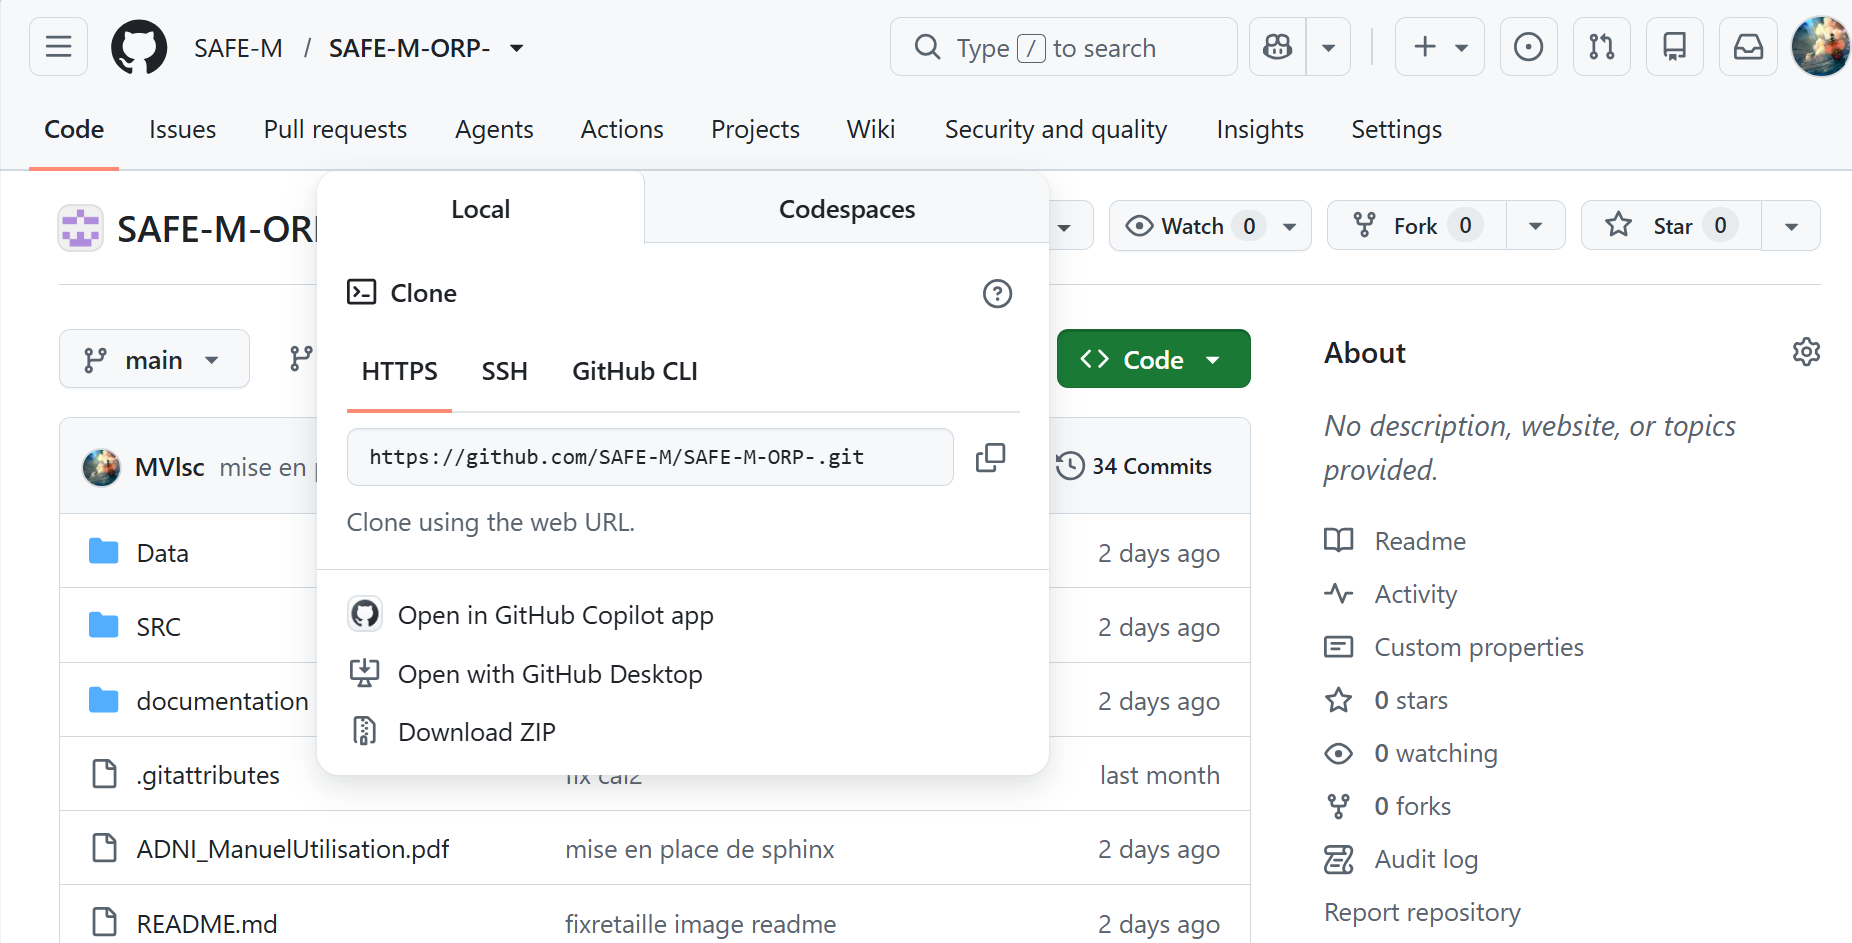
\includegraphics[width = 0.8\textwidth]{figures/git clone.png}
\caption{Copier/coller le lien en cliquant sur code.}
\end{center}
Le dossier est alors chargé sur l’ordinateur de manière locale. Une fois le dossier chargé vous pouvez
vérifier le contenu du dossier en le comparant avec le dossier sur le site github. Le programme et toutes
ses composantes sont alors chargées, vous pouvez dès lors utiliser les pH-mètres.

La figure ci-dessus montre le boîtier SAFE-M-ORP composé de :
\begin{enumerate}
    \item Prise et branchement d’alimentation du Potentiomètre
    \item Sonde température PT100
    \item Sonde ORP
\item Prise
\end{enumerate}

\subsection{Matériel nécessaire}

\begin{itemize}
    \item Carte Arduino
    \item Sonde ORP
    \item Sonde PT100
\end{itemize}
\newpage
\subsection{Connexion boîtier / Ordinateur}
Le code contenu dans le dossier "SRC/Mesure.py"  contient une fonction permettant d'établir la connexion série avec l'Arduino. L'utilisateur
peut choisir de fournir un port manuellement, sinon, grâce à une reconnaissance de nom de port, 
le programme va sélectionner automatiquement le nom relié à l'Arduino. 
Un filtre pour reconnaître les ports Linux ou Windows a été mis en place et présenté dans l'annexe \ref{connexion_port}.


Texte d'introduction du chapitre Installation.

\section{Calibration}
\begin{textblock*}{3mm}(180mm, 5mm)

\includegraphics[width=30 mm]{figures/LOGO-SAFE-M.png}
\end{textblock*}
\subsection{Protocole}

Description du protocole de calibration à deux points.

\begin{lstlisting}[language=Python]
def data(s, N=None, time_inter=0.08):
    T, V, t_temps = [], [], []
    return T, V, t_temps
\end{lstlisting}

\section{Mesures}
\begin{textblock*}{3mm}(180mm, 5mm)

\includegraphics[width=30 mm]{figures/LOGO-SAFE-M.png}
\end{textblock*}
Texte du chapitre Mesures.

\end{document}